\documentclass[12pt,a4paper]{article}
\usepackage[utf8]{vietnam}
\usepackage{amsmath}
\usepackage{amsfonts}
\usepackage{xcolor}
\usepackage{titlesec}
\usepackage{mdframed}
\usepackage{amssymb}
\usepackage{graphicx}
\usepackage{float}
\usepackage{tablefootnote}
\usepackage{adjustbox}
\usepackage{multirow}
\usepackage{pgfplots}
\usepackage{mathrsfs}
\usetikzlibrary{arrows}
\usepackage{fancyhdr}
\pagestyle{fancy}
\pagestyle{empty}
\usepackage{cases} 
\usepackage[left=2cm,right=2cm,top=2cm,bottom=2cm]{geometry}
\author{Nguyễn Văn Lộc}
\newmdenv[linecolor=black,skipabove=\topsep,skipbelow=\topsep,
leftmargin=-5pt,rightmargin=-5pt,
innerleftmargin=5pt,innerrightmargin=5pt]{mybox}
\begin{document}
\fancyhf{}
\lhead{}
\chead{}
\rhead{}
\cfoot{\thepage}
\rfoot{}
\lfoot{}
\pagestyle{fancy}
\begin{flushleft}
\begin{mybox}
\textbf{Họ và tên:} Nguyễn Văn Lộc\\
\textbf{MSSV:} 20120131\\ 
\textbf{Lớp:} 20CTT1TN\\
\textbf{Ca:} Ca 1 (7h30) sáng thứ 4
\end{mybox}
\end{flushleft}
\begin{center}
\textbf{BÀI GIỮA KÌ THỰC HÀNH VI TÍCH PHÂN 2B}
\end{center}
\textbf{Câu 1.}\\
\begin{mybox}
(a) Tìm cực trị của hàm \(f\left( {x,y} \right) = xy\left( {1 - x - y} \right).\) \\
\end{mybox}
\[f\left( {x,y} \right) = xy\left( {1 - x - y} \right)\]
\[ \Leftrightarrow f\left( {x,y} \right) = xy - {x^2}y - x{y^2}.\]
\[{f_x} = \frac{{\partial f}}{{\partial x}} = y - 2xy - {y^2}.\]
\[{f_y} = \frac{{\partial f}}{{\partial y}} = x - 2xy - {x^2}.\]
\[{f_{xx}} = \frac{\partial }{{\partial x}}\left( {{f_x}} \right) = \frac{\partial }{{\partial x}}\left( {y - 2xy - {y^2}} \right) =  - 2y.\]
\[{f_{yy}} = \frac{\partial }{{\partial y}}\left( {{f_y}} \right) = \frac{\partial }{{\partial y}}\left( {x - 2xy - {x^2}} \right) =  - 2x.\]
\[{f_{xy}} = \frac{\partial }{{\partial y}}\left( {{f_x}} \right) = \frac{\partial }{{\partial y}}\left( {y - 2xy - {y^2}} \right) = 1 - 2x - 2y.\]
Xét \(D = {f_{xx}}{f_{yy}} - {\left( {{f_{xy}}} \right)^2} = 4xy - {\left( {1 - 2x - 2y} \right)^2}.\)\\
Xét hệ phương trình:
\begin{equation} 
\left\{ \begin{gathered}
  {f_x} = 0 \hfill \\
  {f_y} = 0 \hfill \\ 
\end{gathered}  \right.
\label{hptdhr}
\end{equation}
\[ \Leftrightarrow \left\{ \begin{gathered}
  y - 2xy - {y^2} = 0 \hfill \\
  x - 2xy - {x^2} = 0 \hfill \\ 
\end{gathered}  \right. \Leftrightarrow \left\{ \begin{gathered}
  y - 2xy - {y^2} = 0 \hfill \\
  \left( {y - x} \right) - \left( {{y^2} - {x^2}} \right) = 0 \hfill \\ 
\end{gathered}  \right. \Leftrightarrow \left\{ \begin{gathered}
  y - 2xy - {y^2} = 0 \hfill \\
  \left( {y - x} \right)\left[ {1 - \left( {y + x} \right)} \right] = 0 \hfill \\ 
\end{gathered}  \right.\]
\[ \Leftrightarrow \left\{ \begin{gathered}
  y - 2xy - {y^2} = 0 \hfill \\
  \left[ \begin{gathered}
  y = x \hfill \\
  y = 1 - x \hfill \\ 
\end{gathered}  \right. \hfill \\ 
\end{gathered}  \right..\]
Trường hợp 1: \[\left\{ \begin{gathered}
  y - 2xy - {y^2} = 0 \hfill \\
  y = x \hfill \\ 
\end{gathered}  \right.\]
Thay \(y = x\) vào \(y - 2xy - y^2 = 0,\) ta được:
\[x - 2x^2 - x^2 = 0\]
\[ \Leftrightarrow x - 3{x^2} = 0\]
\[ \Leftrightarrow \left[ \begin{gathered}
  x = 0 \hfill \\
  x = \frac{1}{3} \hfill \\ 
\end{gathered}  \right. \Leftrightarrow \left[ \begin{gathered}
  \left( {x,y} \right) = \left( {0,0} \right) \hfill \\
  \left( {x,y} \right) = \left( {\frac{1}{3},\frac{1}{3}} \right) \hfill \\ 
\end{gathered}  \right..\]
Trường hợp 2: \[\left\{ \begin{gathered}
  y - 2xy - {y^2} = 0 \hfill \\
  y = 1 - x \hfill \\ 
\end{gathered}  \right.\]
Thay \(y = 1 - x\) vào \(y - 2xy - y^2 = 0,\) ta được:
\[\begin{gathered}
  1 - x - 2x\left( {1 - x} \right) - {\left( {1 - x} \right)^2} = 0 \hfill \\
   \Leftrightarrow {x^2} - x = 0 \hfill \\
   \Leftrightarrow \left[ \begin{gathered}
  x = 0 \hfill \\
  x = 1 \hfill \\ 
\end{gathered}  \right. \Leftrightarrow \left[ \begin{gathered}
  \left( {x,y} \right) = \left( {0,1} \right) \hfill \\
  \left( {x,y} \right) = \left( {1,0} \right) \hfill \\ 
\end{gathered}  \right.. \hfill \\ 
\end{gathered} \]
Vậy hệ (\ref{hptdhr}) có 4 nghiệm là \(\left( {x,y} \right) = \left( {0,0} \right),\left( {x,y} \right) = \left( {\frac{1}{3},\frac{1}{3}} \right),\left( {x,y} \right) = \left( {0,1} \right),\left( {x,y} \right) = \left( {1,0} \right).\)
Xét các nghiệm của hệ phương trình:
\begin{itemize}
\item \(\left( {x,y} \right) = \left( {0,0} \right)\) có \(D\left( {0,0} \right) =  - 1 < 0\) nên không là điểm cực trị của hàm \(f.\)
\item  \(\left( {x,y} \right) = \left( {\frac{1}{3},\frac{1}{3}} \right)\) có
\[\left\{ \begin{gathered}
  D\left( {\frac{1}{3},\frac{1}{3}} \right) = \frac{1}{3} > 0 \hfill \\
  {f_{xx}}\left( {\frac{1}{3},\frac{1}{3}} \right) =  - \frac{2}{3} < 0 \hfill \\ 
\end{gathered}  \right.\] nên là điểm cực đại của hàm \(f.\)
\item \(\left( {x,y} \right) = \left( {0,1} \right)\) có \(D\left( {0,1} \right) =  - 1 < 0\) nên không là điểm cực trị của hàm \(f.\)
\item \(\left( {x,y} \right) = \left( {1,0} \right)\) có \(D\left( {1,0} \right) =  - 1 < 0\) nên không là điểm cực trị của hàm \(f.\)
\end{itemize}
Vậy hàm \(f\) có một điểm cực đại là \(\left( x, y \right) = \left( \frac{1}{3}, \frac{1}{3} \right).\)\\
 Giá trị cực đại của hàm \(f\) là \(f\left( {\frac{1}{3},\frac{1}{3}} \right) = \frac{1}{{27}}.\)
\begin{mybox}
(b) Chỉ ra rằng mọi mặt tiếp xúc với mặt \(\left( S \right):{x^2} + {y^2} - {z^2} = 2y - 2z\) đều đi qua một điểm cố định \(I.\) Hãy tìm điểm \(I.\)
\end{mybox} 
Xét hàm \(F\) định bởi \(F\left( {x,y,z} \right) = {x^2} + {y^2} - {z^2} - 2y + 2z.\)\\
Xét điểm \(A\left( {{x_0},{y_0},{z_0}} \right) \in \left( S \right) \Leftrightarrow F\left( {{x_0},{y_0},{z_0}} \right) = 0.\)\\
Mặt phẳng \(\left( P \right)\) tiếp xúc với \(\left( S \right)\) tại điểm \(A\) có phương trình:
\[\left( P \right):\nabla F\left( {{x_0},{y_0},{z_0}} \right) \cdot \left\langle {x - {x_0},y - {y_0},z - {z_0}} \right\rangle  = 0\]
\[ \Leftrightarrow \left\langle {2{x_0},2{y_0} - 2, - 2{z_0} + 2} \right\rangle  \cdot \left\langle {x - {x_0},y - {y_0},z - {z_0}} \right\rangle  = 0\]
\begin{equation}
 \Leftrightarrow 2{x_0}\left( {x - {x_0}} \right) + \left( {2{y_0} - 2} \right)\left( {y - {y_0}} \right) + \left( { - 2{z_0} + 2} \right)\left( {z - {z_0}} \right) = 0
\end{equation} \label{ptmp}
Ta sẽ chứng minh mặt phẳng \(P\) luôn đi qua điểm \(C\left( {0,1,1} \right) \in \left( S \right).\) 
\begin{itemize}
\item Nếu \(A \equiv C\) thì ta có đpcm.
\item Nếu \(A \not \equiv C\):
Phương trình mặt phẳng \(\left( P \right)\) tương đương với:
\[\left( { - 2x_0^2 - 2y_0^2 + 2z_0^2 + 2{y_0} - 2{z_0}} \right) + 2{x_0}x + \left( {2{y_0} - 2} \right)y + \left( { - 2{z_0} + 2} \right)z = 0,\forall \left( {{x_0},{y_0},{z_0}} \right) \ne \left( {0,1,1} \right)\]
\[ \Leftrightarrow \left( { - 2x_0^2 - 2y_0^2 + 2z_0^2 + 4{y_0} - 4{z_0}} \right) + 2{x_0}x + \left[ {\left( {2{y_0} - 2} \right)y - 2{y_0}} \right] + \left[ {\left( { - 2{z_0} + 2} \right)z + 2{z_0}} \right] = 0,\]
\[\forall \left( {{x_0},{y_0},{z_0}} \right) \ne \left( {0,1,1} \right)\]
\[ \Leftrightarrow 2F\left( {{x_0},{y_0},{z_0}} \right) + 2{x_0}x + \left[ {\left( {2{y_0} - 2} \right)y - \left( {2{y_0} - 2} \right)} \right] + \left[ {\left( { - 2{z_0} + 2} \right)z - \left( {2{z_0} + 2} \right)} \right] = 0,\]
\[\forall \left( {{x_0},{y_0},{z_0}} \right) \ne \left( {0,1,1} \right)\]
\[ \Leftrightarrow 2{x_0}x + \left( {2{y_0} - 2} \right)\left( {y - 1} \right) + \left( { - 2{z_0} + 2} \right)\left( {z - 1} \right) = 0,\forall \left( {{x_0},{y_0},{z_0}} \right) \ne \left( {0,1,1} \right)\]
\[ \Leftrightarrow \left\{ \begin{gathered}
  x = 0 \hfill \\
  y - 1 = 0 \hfill \\
  z - 1 = 0 \hfill \\ 
\end{gathered}  \right. \Leftrightarrow \left\{ \begin{gathered}
  x = 0 \hfill \\
  y = 1 \hfill \\
  z = 1 \hfill \\ 
\end{gathered}  \right.\]
\end{itemize}
Vậy mặt phẳng \(\left( P \right)\) luôn đi qua điểm \(I\left( {0,1,1} \right).\)\\
\textbf{Câu 2.}
\begin{mybox}
Tính tích phân lặp \[I = \int\limits_0^8 {\int\limits_{\sqrt[3]{y}}^2 {\sqrt {{x^4} + 1} } dxdy.} \]
\end{mybox}
\[\left\{ \begin{gathered}
  0 \leqslant y \leqslant 8 \hfill \\
  \sqrt[3]{y} \leqslant x \leqslant 2 \hfill \\ 
\end{gathered}  \right. \Rightarrow \left\{ \begin{gathered}
  0 \leqslant y \leqslant {x^3} \hfill \\
  0 \leqslant x \leqslant 2 \hfill \\ 
\end{gathered}  \right.\]
Vậy \[I = \int\limits_0^8 {\int\limits_{\sqrt[3]{y}}^2 {\sqrt {{x^4} + 1} dxdy} } \]
\[ \Rightarrow I = \int\limits_0^{{x^3}} {\int\limits_0^2 {\sqrt {{x^4} + 1} dxdy} } \]
\[ \Rightarrow I = \int\limits_0^2 {\left( {\int\limits_0^{{x^3}} {\sqrt {{x^4} + 1} dy} } \right)dx} \]
\[ \Rightarrow I = \int\limits_0^2 {\left( {\left. {y\sqrt {{x^4} + 1} } \right|_{y = 0}^{y = {x^3}}} \right)dx} \]
\[ \Rightarrow I = \int\limits_0^2 {{x^3}\sqrt {{x^4} + 1} dx} \]
Đặt \(t = \sqrt {{x^4} + 1}  \Rightarrow {t^2} = {x^4} + 1 \Rightarrow 2tdt = 4{x^3}dx \Rightarrow {x^3}dx = \frac{1}{2}tdt\)
\[ \Rightarrow I = \int\limits_1^{\sqrt {17} } {\frac{1}{2}t \cdot tdt}  = \left. {\frac{{{t^3}}}{6}} \right|_{t = 1}^{t = \sqrt {17} } = \frac{{17\sqrt {17}  - 1}}{6}.\]
\textbf{Câu 3.}
\begin{mybox}
Tính tích phân \(\int_C {\left( {2{x^2} + y} \right)dx - xdy,} \) trong đó \(C\) là biên của miền \(D\) và được định hướng âm, với \(D\) là miền giới hạn bởi các đường \(y = x^2\) và \(y = x.\)
\end{mybox}
\begin{center}
\begin{figure}[H]
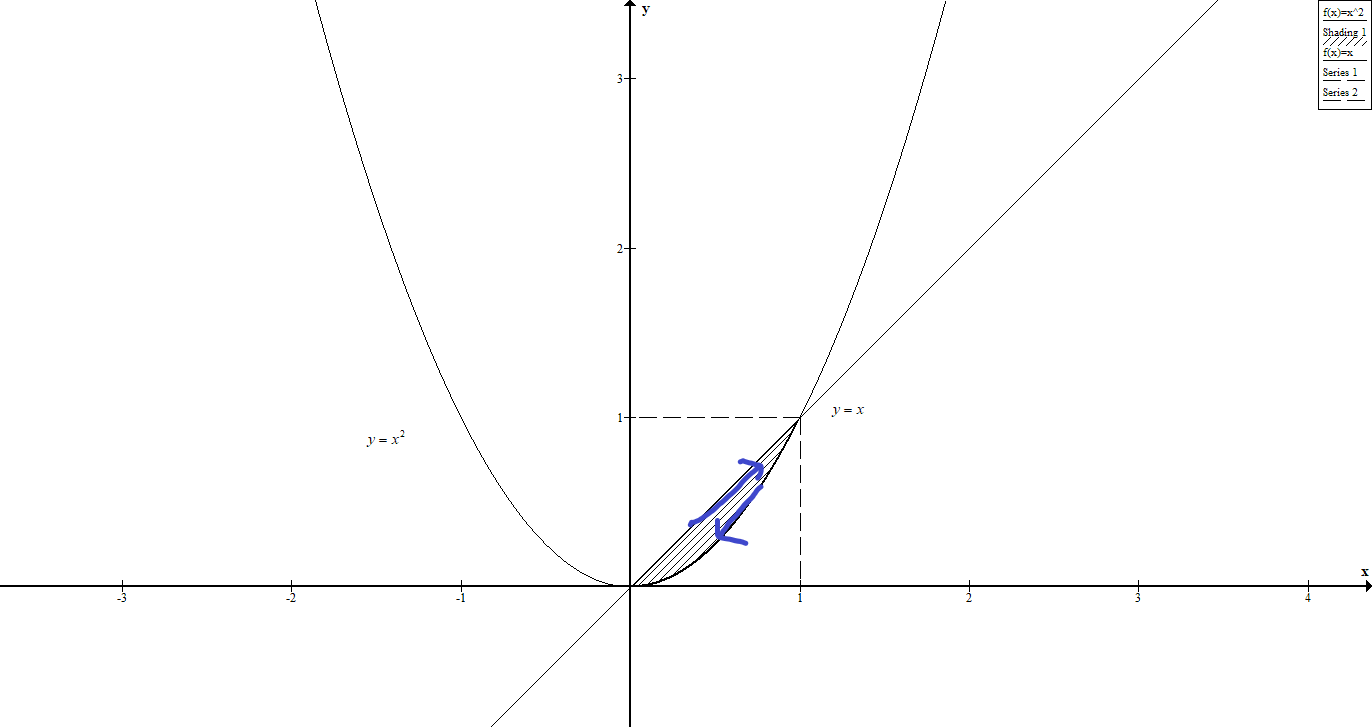
\includegraphics[scale=0.4]{anhgk1}
\end{figure}
\end{center}
Xét phương trình hoành độ giao điểm \(y = x^2\) và \(y = x.\)
\[{x^2} = x\]
\[ \Leftrightarrow \left[ \begin{gathered}
  x = 0 \hfill \\
  x = 1 \hfill \\ 
\end{gathered}  \right..\]
Vậy đồ thị hàm số \(y = x^2\) và đồ thị hàm số \(y = x\) cắt nhau tại 2 điểm \(A \left( {0,0} \right)\) và \(B \left( {1, 1} \right).\)\\
Gọi \(C_1\) là phần đồ thị hàm số \(y = x^2\) từ \(0\) đến \(1,\) \(C_2\) là phần đồ thị hàm số \(y = x\) từ \(0\) đến \(1.\)\\
Hướng âm trên \(C_1\) là từ \(B\) đến \(A,\) còn hướng âm trên \(C_2\) là từ \(A\) đến \(B.\)\\
Một tham số hóa cho đường cong \(\left( {{C_1}} \right)\) là \(x = -t,y = {t^2}\) với \(t \in \left[ {-1,0} \right].\)\\
Một tham số hóa cho đường cong \(\left( {{C_2}} \right)\) là \(x = x,y = x\) với \(x \in \left[ {0,1} \right].\)
\[I = \int_C {\left( {2{x^2} + y} \right)dx - xdy} \]
\[ = \int_{{C_1}} {\left( {2{x^2} + y} \right)dx - xdy}  + \int_{{C_2}} {\left( {2{x^2} + y} \right)dx - xdy} \]
\[ = \int\limits_{ - 1}^0 {\left( {2{t^2} + {t^2}} \right)\left( { - dt} \right) + t \cdot 2tdt + \int\limits_0^1 {\left( {2{x^2} + x} \right)dx - xdx} } \]
\[ = \int\limits_{ - 1}^0 {\left( { - {t^2}} \right)dt + \int\limits_0^1 {2{x^2}dx} }  = \frac{1}{3}.\]
\textbf{Câu 4.}
\begin{mybox}
Carbon \(C^{14}\) là một chất phóng xạ. Theo mô hình hóa học, số lượng nguyên từ bị phân rã trong một đơn vị thời gian trên một đơn vị số lượng nguyên tử là không đổi. Như vậy, nếu gọi \(C \left( t \right)\) là số lượng nguyên tử ở thời điểm \(t\) (năm) tính từ lúc Carbon \(C^{14}\) bắt đầu phân rã, \(t > 0,\) thì \\
\[\frac{{C'\left( t \right)}}{{C\left( t \right)}} = k,\forall t \geqslant 0,\]
trong đó \(k\) là một hằng số thực.\\
(a). Chứng tỏ \[C\left( t \right) = C\left( 0 \right){e^{kt}}.\]
(b). Người ta biết \(C^{14}\) phân rã theo quy luật giảm đi phân nửa sau \(5730\) năm. Từ đó, hãy kiểm rằng \(k \approx -0,00012.\) Hãy cho biết đơn vị của \(k.\)
\end{mybox}
(a). \[\frac{{C'\left( t \right)}}{{C\left( t \right)}} = k,\forall t \ge 0\]
\[ \Leftrightarrow C'\left( t \right) = k \cdot C\left( t \right),\forall t \ge 0\]
\[ \Leftrightarrow C'\left( t \right) - k \cdot C\left( t \right) = 0,\forall t \ge 0\]
\[ \Leftrightarrow {e^{ - kt}}C'\left( t \right) - k \cdot {e^{ - kt}} \cdot C\left( t \right) = 0,\forall t \ge 0\]
\[ \Leftrightarrow {\left( {{e^{ - kt}} \cdot C\left( t \right)} \right)^\prime } = 0,\forall t \ge 0\]
\[ \Leftrightarrow \int {{{\left( {{e^{ - kt}} \cdot C\left( t \right)} \right)}^\prime }dt = \int {0dt,} } \forall t \ge 0\]
\[ \Leftrightarrow {e^{ - kt}} \cdot C\left( t \right) = M,\left( {M = const} \right),\forall t \ge 0\]
\begin{equation}  \label{ptvp}
 \Leftrightarrow C\left( t \right) = M \cdot {e^{kt}},\forall t \ge 0
\end{equation} 
Thay \(t = 0\) vào (\ref{ptvp}), ta được:
\[C\left( 0 \right) = M \cdot {e^0} \Rightarrow M = C\left( 0 \right).\]
Vậy \[C\left( t \right) = C\left( 0 \right){e^{kt}}.\]
(b). \(C^{14}\) phân rã theo quy luật số lượng giảm đi một nửa sau \(5730\) năm, do đó:
\[C\left( {5730} \right) = \frac{1}{2}C\left( 0 \right)\]
\[ \Leftrightarrow C\left( 0 \right) \cdot {e^{k \cdot 5730}} = \frac{1}{2}C\left( 0 \right), \left( C \left( 0 \right) \ne 0 \right)\]
\[ \Leftrightarrow {e^{5730k}} = \frac{1}{2}\]
\[ \Leftrightarrow 5730k = \ln \left( {\frac{1}{2}} \right) =  - \ln 2\]
\[ \Leftrightarrow k =  - \frac{{\ln 2}}{{5730}} \approx  - 0,00012\]
Đơn vị tính của \(k:\) năm\(^-1\)
\end{document}